
\subsection*{1.}

\paragraph{a.} Si \( x \) est la longueur des deux côtés perpendiculaires au mur, l'autre côté a pour longueur \( 28 - 2x \).

Donc l'aire de l'enclos est :
\[
\mathcal{A}(x) = x(28 - 2x) = 28x - 2x^2.
\]

\paragraph{b.} On a :
\begin{align*}
\mathcal{A}(x) &= -2x^2 + 28x \\
&= -2 \left(x^2 - 14x\right) \\
&= -2 \left[(x - 7)^2 - 49\right] \\
&= -2(x - 7)^2 + 98.
\end{align*}

\subsection*{2.}

Le coefficient de \( x^2 \) étant négatif, la concavité est tournée vers le bas : on élimine donc \( \mathcal{C}_1 \) et \( \mathcal{C}_4 \).

D'autre part, on a \( \mathcal{A}(0) = 0 \) : la courbe représentative doit contenir l'origine. La bonne courbe est donc \( \mathcal{C}_2 \).

\subsection*{3.}

On voit que le maximum est atteint pour \( x = 7 \), ce maximum étant égal à 98.

La fonction est donc croissante sur \( [0 \,;\, 7] \), puis décroissante sur \( [7 \,;\, 28] \).

\begin{center}
\begin{tikzpicture}
\tkzTabInit[lgt=3.5, espcl=4]{$x$ / 1, {$f(x)$} / 2}{${0}$, ${7}$, ${14}$}
\tkzTabVar{-/{$0$},+/{$98$},-/{$0$}}{/}
\end{tikzpicture}
\end{center}

\subsection*{4.}

On a vu que l'aire maximale est obtenue pour \( x = 7 \) avec une aire maximale de \( 98 \, \text{m}^2 \).

